%!TEX root = ./main.tex
%!TEX program = xelatex
% =====================================================================
%  02 - QUÁ TRÌNH THIẾT KẾ PHẦN CỨNG
% =====================================================================
\chapter{Quá trình thiết kế phần cứng}
\label{ch:thietke}

\section{Quy trình thiết kế tổng thể}

Phần cứng của \proj{} được phát triển theo quy trình ``chữ V'' rút gọn: bắt đầu từ yêu cầu chức năng, đi xuống thiết kế chi tiết từng khối, sau đó đi lên qua chế tạo, lắp ráp và kiểm thử từng khối trước khi tích hợp toàn hệ thống (Hình~\ref{fig:quytrinh}). Toàn bộ thiết kế điện tử được thực hiện trên phần mềm mã nguồn mở \textbf{KiCad}.

\begin{figure}[H]
\centering
\resizebox{\linewidth}{!}{%
\begin{tikzpicture}[
  st/.style={draw=blk,thick,rounded corners=3pt,fill=blkfill,minimum width=34mm,minimum height=9mm,align=center,font=\small},
  ar/.style={-{Stealth[length=2.5mm]},thick}]
  \node[st] (a) at (0,0) {1. Xác định yêu cầu};
  \node[st] (b) at (1.4,-1.3) {2. Kiến trúc \& sơ đồ khối};
  \node[st] (c) at (2.8,-2.6) {3. Chọn linh kiện};
  \node[st] (d) at (4.2,-3.9) {4. Sơ đồ nguyên lý};
  \node[st,fill=swfill] (e) at (7,-5.2) {5. Bố trí \& đi dây PCB};
  \node[st] (f) at (9.8,-3.9) {6. DRC, xuất Gerber};
  \node[st] (g) at (11.2,-2.6) {7. Gia công \& hàn};
  \node[st] (h) at (12.6,-1.3) {8. Kiểm tra từng khối};
  \node[st] (i) at (14,0) {9. Tích hợp firmware};
  \foreach \x/\y in {a/b,b/c,c/d,d/e,e/f,f/g,g/h,h/i} \draw[ar] (\x) -- (\y);
  \draw[ar,dashed,gray] (h.north west) to[bend right=20] node[above,font=\scriptsize]{sửa lỗi} (d.north east);
\end{tikzpicture}}
\caption{Quy trình thiết kế phần cứng \proj}
\label{fig:quytrinh}
\end{figure}

\subsection{Yêu cầu thiết kế}
Từ mục tiêu đề tài, nhóm đặt ra các yêu cầu sau làm cơ sở cho mọi quyết định thiết kế:
\begin{enumerate}[label=\textbf{R\arabic*.}]
  \item Dùng \textbf{một nguồn duy nhất} \SI{12}{\volt} cho cả động cơ và mạch điều khiển.
  \item Điều khiển động cơ DC \SI{12}{\volt} \textbf{hai chiều}, dòng tới khoảng \SI{1}{\ampere}.
  \item Đọc encoder, \textbf{điều khiển vòng kín} bằng PID.
  \item Đặt tốc độ bằng \textbf{chiết áp} hoặc \textbf{UART}.
  \item Có \textbf{giao diện người dùng}: nút nhấn, LED, màn hình.
  \item \textbf{Bảo vệ} khi cắm ngược nguồn; ngắt tầng công suất khi dừng.
  \item Nạp được chương trình \textbf{không cần bootloader} (ISP), có điểm đo (test point) cho việc gỡ lỗi.
  \item Bo mạch \textbf{nhỏ gọn}, 2 lớp, linh kiện dán (SMD) phổ biến, dễ đặt gia công.
\end{enumerate}

\section{Lựa chọn linh kiện}

\subsection{Vi điều khiển: ATmega88PA}
\begin{table}[H]
\centering\small
\caption{So sánh các phương án vi điều khiển}
\label{tab:sosanh_mcu}
\begin{tabularx}{\linewidth}{@{}l>{\centering\arraybackslash}X>{\centering\arraybackslash}X>{\centering\arraybackslash}X@{}}
\toprule
\textbf{Tiêu chí} & \textbf{ATmega88PA} & \textbf{ATmega328P} & \textbf{STM32F103}\\
\midrule
Kiến trúc & AVR 8-bit & AVR 8-bit & ARM Cortex-M3 32-bit\\
Flash / SRAM & 8\,KB / 1\,KB & 32\,KB / 2\,KB & 64\,KB / 20\,KB\\
Điện áp & \SIrange{1.8}{5.5}{\volt} & \SIrange{1.8}{5.5}{\volt} & \SIrange{2}{3.6}{\volt}\\
Bộ giải mã encoder phần cứng & Không & Không & Có\\
Phù hợp nội dung học phần & Rất cao & Rất cao & Trung bình\\
Giá thành & Thấp & Trung bình & Trung bình\\
\bottomrule
\end{tabularx}
\end{table}

\begin{figure}[H]
\centering
\begin{subfigure}{0.49\linewidth}\centering\hinh[\linewidth]{figures/ATmega88PA_Front.jpg}{Ảnh MCU ATmega88PA mặt trên}\caption{Mặt trên}\end{subfigure}
\hfill
\begin{subfigure}{0.49\linewidth}\centering\hinh[\linewidth]{figures/ATmega88PA_Back.jpg}{Ảnh MCU ATmega88PA mặt dưới}\caption{Mặt dưới}\end{subfigure}
\caption{MCU ATmega88PA}
\label{fig:ATmega88PA}
\end{figure}

Nhóm chọn \textbf{ATmega88PA} vì: (i) cùng họ AVR với nội dung giảng dạy, tương thích chân với ATmega328P nên có thể nâng cấp bộ nhớ mà không sửa PCB; (ii) hoạt động ở \SI{5}{\volt}, tương thích trực tiếp với encoder, nút nhấn và đầu vào logic của DRV8220; (iii) chi phí thấp. Bộ nhớ 8\,KB Flash là một \emph{thử thách có chủ đích}: buộc nhóm phải viết firmware tối giản, thao tác trực tiếp thanh ghi thay vì dùng thư viện Arduino, vốn rất tốn dung lượng flash.

\subsection{IC Cầu H: DRV8220}
\begin{table}[H]
\centering\small
\caption{So sánh các phương án cầu H}
\label{tab:sosanh_drv}
\begin{tabularx}{\linewidth}{@{}l>{\centering\arraybackslash}X>{\centering\arraybackslash}X>{\centering\arraybackslash}X@{}}
\toprule
\textbf{Tiêu chí} & \textbf{L298N} & \textbf{TB6612FNG} & \textbf{DRV8220}\\
\midrule
Công nghệ & BJT & MOSFET & MOSFET\\
Điện áp động cơ & \SIrange{5}{46}{\volt} & \SIrange{2.5}{13.5}{\volt} & \SIrange{4.5}{18}{\volt}\\
Sụt áp / $R_{DS(on)}$ & $\sim$\SI{2}{\volt} & $\sim$\SI{0.5}{\ohm} & $\sim$\SI{1}{\ohm} (HS+LS)\\
Bảo vệ tích hợp & Không & Nhiệt & OCP, TSD, UVLO\\
Kích thước vỏ & Multiwatt-15 & SSOP-24 & WSON-8 2\,$\times$\,2\,mm\\
Chế độ ngủ & Không & Có & Có (dòng nA)\\
\bottomrule
\end{tabularx}
\end{table}

\begin{figure}[H]
\centering
\begin{subfigure}{0.49\linewidth}\centering\hinh[\linewidth]{figures/DRV8220DSG_Front.jpg}{Ảnh DRV8220 mặt trên}\caption{Mặt trên}\end{subfigure}
\hfill
\begin{subfigure}{0.49\linewidth}\centering\hinh[\linewidth]{figures/DRV8220DSG_Back.jpg}{Ảnh DRV8220 mặt dưới}\caption{Mặt dưới}\end{subfigure}
\caption{IC cầu H DRV8220}
\label{fig:drv8220}
\end{figure}

\textbf{DRV8220} được chọn vì phù hợp nguồn \SI{12}{\volt} (TB6612 chỉ tới \SI{13.5}{\volt}, sát giới hạn), có đầy đủ bảo vệ quá dòng, quá nhiệt, thấp áp, kích thước rất nhỏ (WSON-8 2x2mm), và có chân \texttt{nSLEEP} để ngắt hẳn tầng công suất -- đáp ứng yêu cầu R6. Ngoài ra, DRV8220 hỗ trợ hai chế độ giao tiếp IN1/IN2 (PWM) và PH/EN, được chọn bằng chân MODE; nhóm bố trí jumper hàn \textbf{JP1} cùng điện trở kéo xuống R10 để có thể chuyển chế độ mà không cần sửa mạch.

\subsection{Nguồn: buck LMR51420 + LDO AP2112K}
Mạch điều khiển cần đường \SI{5}{\volt} (MCU, encoder, logic) và \SI{3.3}{\volt} (màn hình TFT). Với dòng tải ước tính \SI{150}{\milli\ampere} trên đường \SI{5}{\volt}, nếu dùng ổn áp tuyến tính 7805 thì công suất tiêu tán:
\begin{equation}
  P_{7805}=(V_{IN}-V_{OUT})\cdot I=(12-5)\times0{,}15=\SI{1.05}{\watt},
\end{equation}
đòi hỏi tản nhiệt và lãng phí khoảng 58\,\% năng lượng. Nhóm chọn IC \textbf{buck LMR51420} (hiệu suất trên 85\,\%, package SOT-23-6, dòng ra tới \SI{2}{\ampere}, phiên bản \texttt{XF} chạy \SI{500}{\kilo\hertz} ở chế độ FPWM để tần số chuyển mạch cố định, dễ lọc nhiễu). Đường \SI{3.3}{\volt} chỉ cấp cho màn hình nên dùng LDO \textbf{AP2112K-3.3} (\SI{600}{\milli\ampere}, sụt áp thấp) nối sau đường \SI{5}{\volt} -- tổn hao chỉ $(5-3{,}3)\times I_{TFT}$, không đáng kể.

\begin{figure}[H]
\centering
\begin{subfigure}{0.49\linewidth}\centering\hinh[\linewidth]{figures/LMR51420.jpg}{Ảnh IC LMR51420}\caption{Ảnh IC LMR51420}\end{subfigure}
\hfill
\begin{subfigure}{0.49\linewidth}\centering\hinh[\linewidth]{figures/AP2112K.jpg}{Ảnh IC AP2112K}\caption{Ảnh IC AP2112K}\end{subfigure}
\caption{IC buck LMR51420 và LDO AP2112K}
\label{fig:lmr51420_ap2112k}
\end{figure}

\subsection{Chống ngược cực: P-MOSFET CSD25404Q3}
\begin{table}[H]
\centering\small
\caption{So sánh các phương án chống ngược cực tại $I=\SI{1}{\ampere}$}
\label{tab:sosanh_rpp}
\begin{tabular}{@{}lccc@{}}
\toprule
\textbf{Phương án} & \textbf{Sụt áp} & \textbf{Tổn hao} & \textbf{Ghi chú}\\
\midrule
Diode chỉnh lưu nối tiếp (1N5819) & $\sim$\SI{0.45}{\volt} & $\sim$\SI{0.45}{\watt} & Đơn giản, tổn hao lớn\\
Diode song song + cầu chì & 0 & 0 & Phải thay cầu chì sau sự cố\\
\textbf{P-MOSFET (CSD25404Q3)} & \textbf{\SI{5.5}{\milli\volt}} & \textbf{\SI{5.5}{\milli\watt}} & Tự phục hồi, gần như không tổn hao\\
\bottomrule
\end{tabular}
\end{table}

\begin{figure}[H]
\centering
\begin{subfigure}{0.45\linewidth}\centering\hinh[\linewidth]{figures/CSD25404Q3_Front.jpg}{Ảnh MOSFET CSD25404Q3}\caption{Mặt trên}\end{subfigure}
\hfill
\begin{subfigure}{0.45\linewidth}\centering\hinh[\linewidth]{figures/CSD25404Q3_Back.jpg}{Ảnh MOSFET CSD25404Q3}\caption{Mặt dưới}\end{subfigure}
\caption{P MOSFET CSD25404Q3}
\label{fig:CSD25404Q3}
\end{figure}

Nguyên lý: khi cắm đúng cực, dòng ban đầu chạy qua diode thân của Q1 làm cực nguồn S lên khoảng \SI{11.3}{\volt}, trong khi cực cổng G được R2 (\SI{100}{\kilo\ohm}) kéo về GND, nên $V_{GS}<0$ và MOSFET dẫn hoàn toàn. Zener \textbf{D1} (\SI{10}{\volt}) kẹp $|V_{GS}|\le\SI{10}{\volt}$, bảo vệ cực cổng (giới hạn $\pm\SI{12}{\volt}$) khi nguồn vào cao. Khi cắm ngược, $V_{GS}\ge0$, diode thân phân cực ngược và MOSFET khóa, mạch phía sau được cách ly.

\subsection{IC chuyển mức logic: TXB0106}

\begin{figure}[H]
\centering
\begin{subfigure}{0.45\linewidth}\centering\hinh[\linewidth]{figures/TXB0106_Front.jpg}{Ảnh IC TXB0106}\caption{Mặt trên}\end{subfigure}
\hfill
\begin{subfigure}{0.45\linewidth}\centering\hinh[\linewidth]{figures/TXB0106_Back.jpg}{Ảnh IC TXB0106}\caption{Mặt dưới}\end{subfigure}
\caption{IC chuyển mức logic TXB0106}
\label{fig:TXB0106}
\end{figure}

Module TFT WeAct ST7735 làm việc ở mức logic \SI{3.3}{\volt}, trong khi ATmega88PA xuất mức \SI{5}{\volt}. Nhóm dùng IC chuyển mức hai chiều tự nhận hướng \textbf{TXB0106} (6 kênh: SCK, MOSI, CS, DC, RST, BL) thay cho cầu phân áp điện trở, nhằm đảm bảo sườn xung SPI \SI{8}{\mega\hertz} sắc nét. Chân OE (tham chiếu theo $V_{CCA}=\SI{3.3}{\volt}$) được cấp qua cầu phân áp R9/R12:
\begin{equation}
  V_{OE}=V_{in}\cdot\frac{R_{12}}{R_9+R_{12}}=5\times\frac{60{,}4}{30{,}1+60{,}4}\approx\SI{3.34}{\volt}.
\end{equation}

\section{Thiết kế sơ đồ nguyên lý}

Sơ đồ nguyên lý được vẽ trên một trang A4, chia thành các vùng khối có tiêu đề theo đúng sơ đồ khối ở Hình~\ref{fig:sodokhoi}: \emph{Reverse Polarity Protection}, \emph{Power}, \emph{MCU}, \emph{IO}, \emph{Motor Driver}, \emph{LEDs}, \emph{Level Shifter}, \emph{Debug/UART/Encoder}. Sơ đồ đầy đủ được trình bày tại Phụ lục~\ref{app:schematic}. Một số tính toán chính:

\begin{figure}[H]
\centering
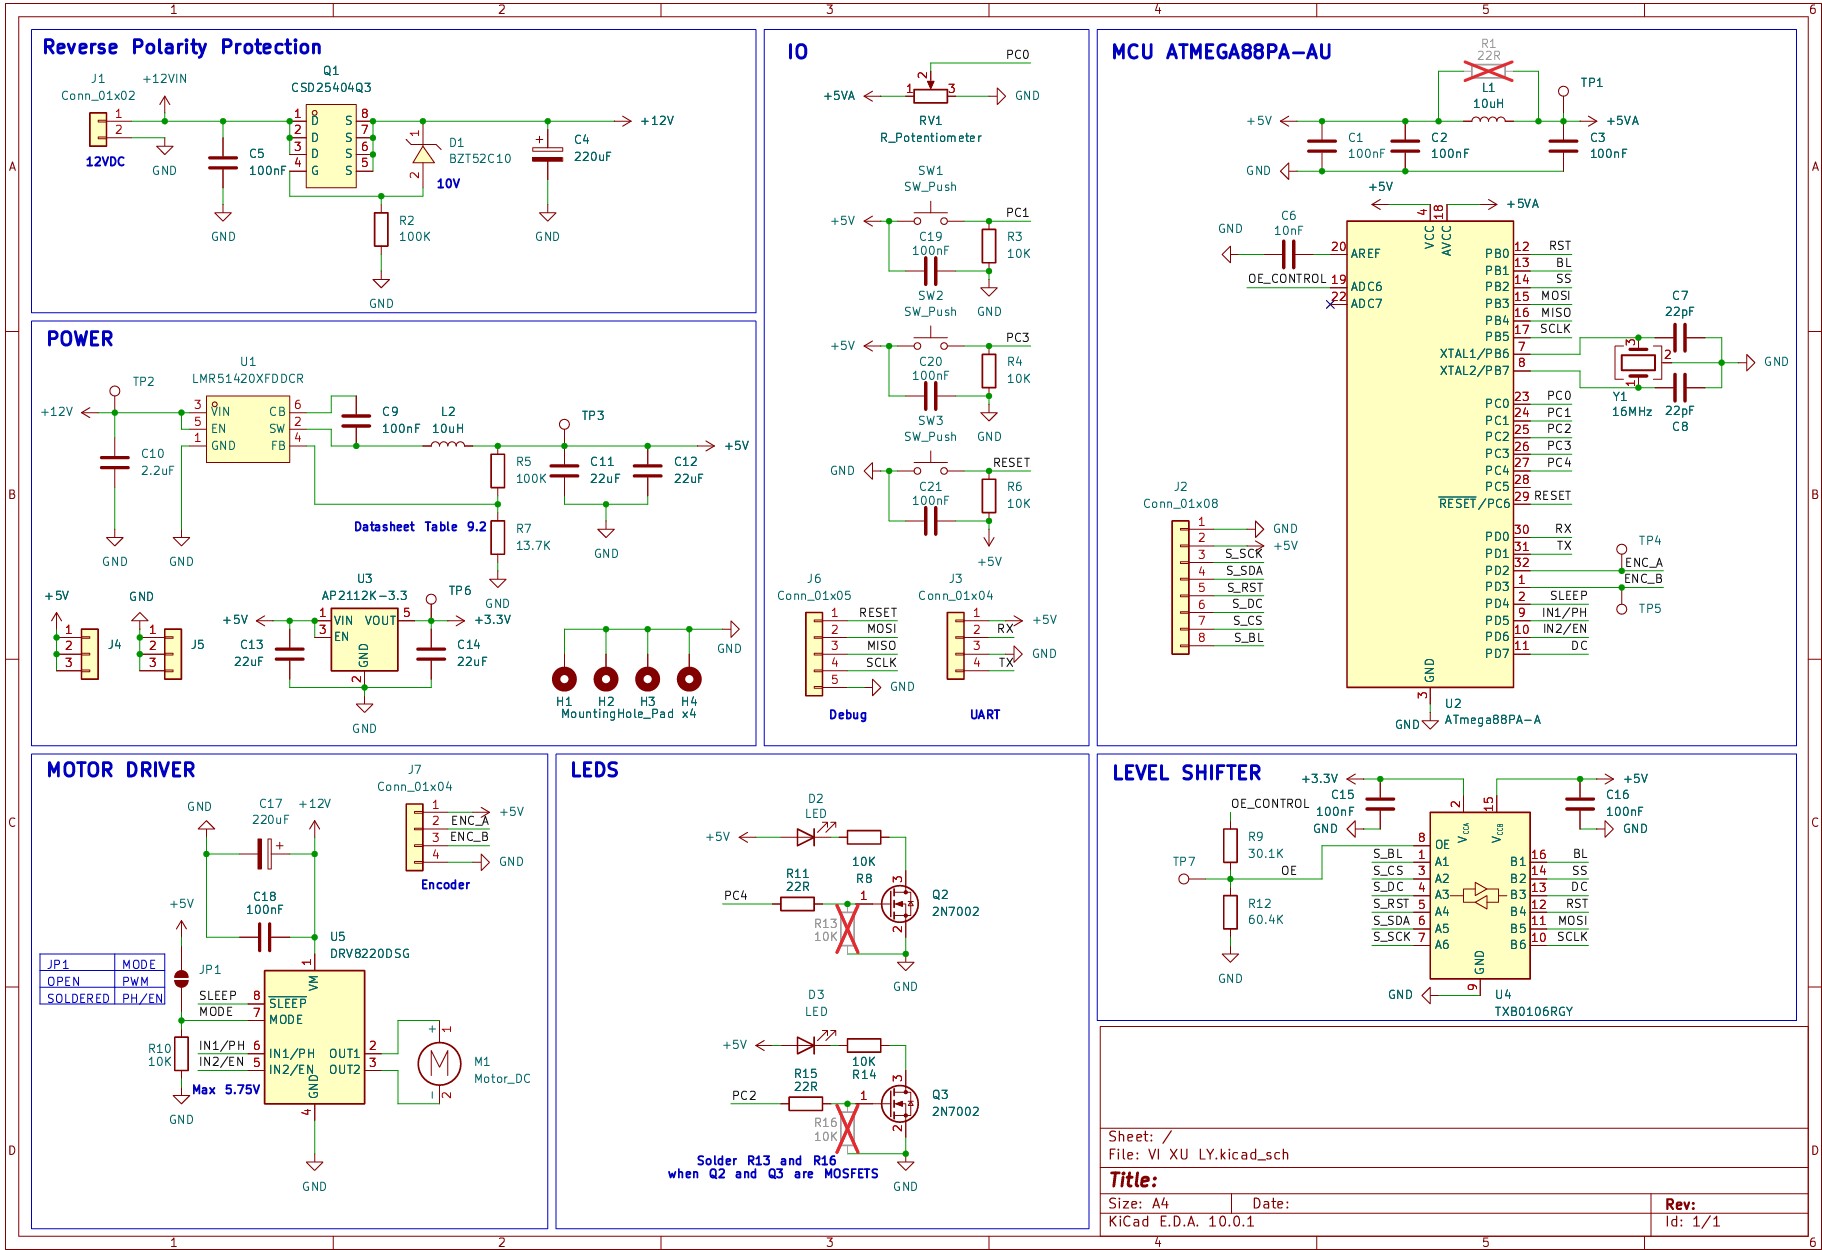
\includegraphics[width=\linewidth]{sch/SCH_PIC.png}
\caption{Sơ đồ nguyên lý \proj}
\label{fig:schematic}
\end{figure}

\paragraph{Mạch chống ngược cực.} P-MOSFET Q1 (CSD25404Q3) được đặt nối tiếp trên đường +12V từ đầu nối J1. Cực cổng được kéo xuống GND qua R2 (\SI{100}{\kilo\ohm}) nên khi cấp nguồn đúng cực, $V_{GS}\approx-\SI{12}{\volt}$ và MOSFET dẫn hoàn toàn; khi cắm ngược cực, $V_{GS}\ge0$ và MOSFET khóa, bảo vệ toàn bộ mạch phía sau. Zener D1 (BZT52C10) kẹp $|V_{GS}|$ ở \SI{10}{\volt}, dưới giới hạn tối đa của Q1. Tụ C5 (\SI{100}{\nano\farad}) và tụ hóa C4 (\SI{220}{\micro\farad}) lọc và dự trữ năng lượng cho bus +12V.

\begin{figure}[H]
\centering
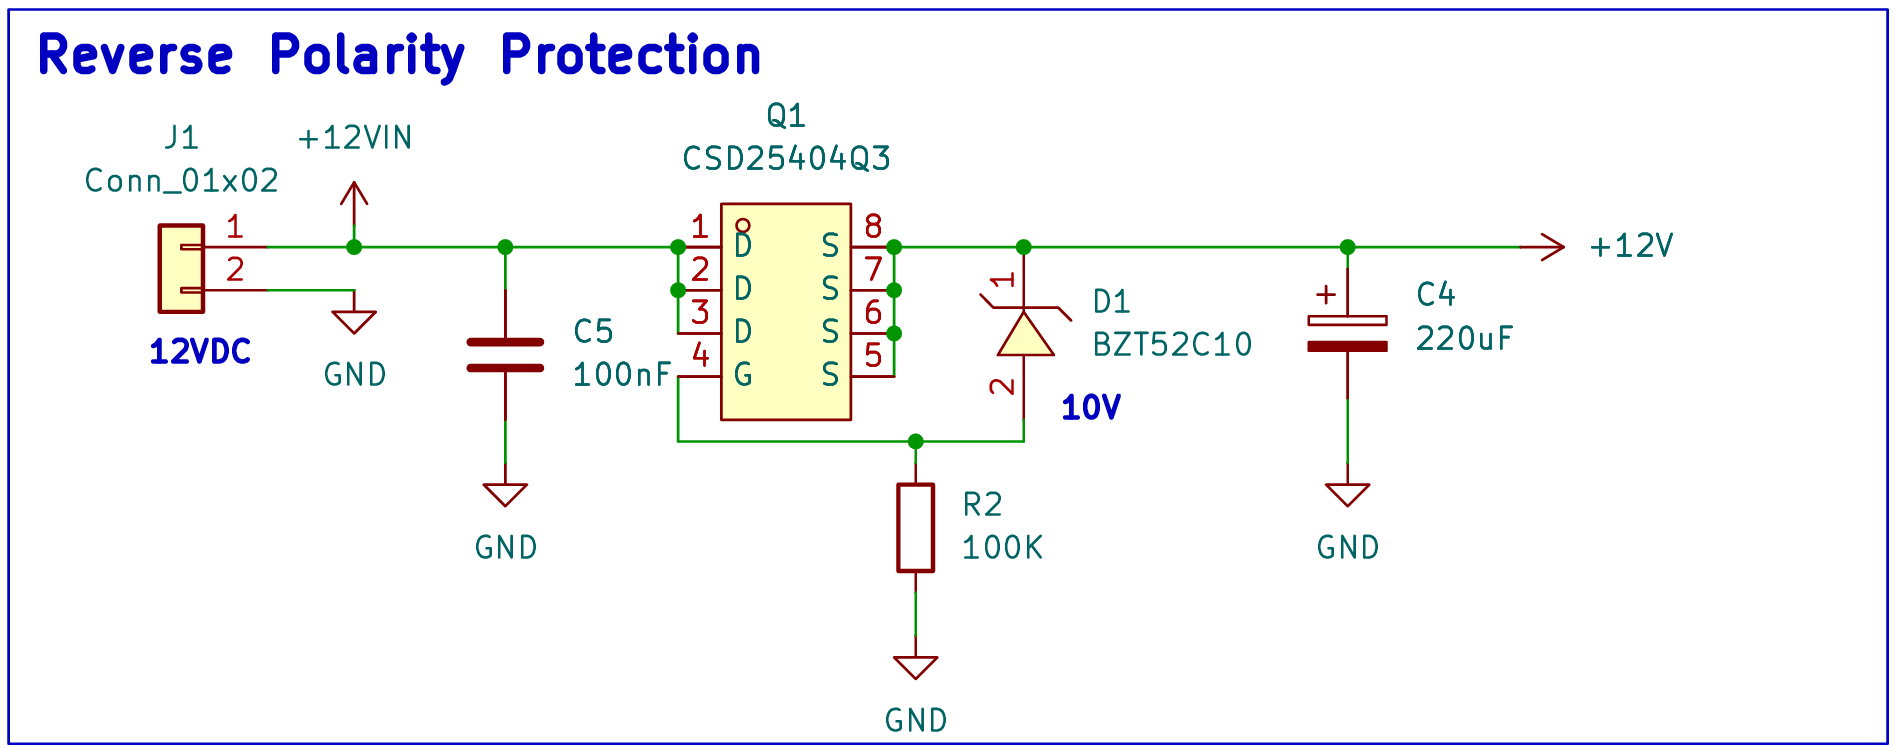
\includegraphics[width=0.9\linewidth]{figures/Reverse_polarity.png}
\caption{Mạch chống ngược cực dùng P-MOSFET CSD25404Q3}
\label{fig:sch_rpp}
\end{figure}

\paragraph{Điện áp ra của buck.} Với $V_{FB}=\SI{0.6}{\volt}$, $R_5=\SI{100}{\kilo\ohm}$ (FB lên +5V), $R_7=\SI{13.7}{\kilo\ohm}$ (FB xuống GND):
\begin{equation}
  V_{OUT}=0{,}6\left(1+\frac{100}{13{,}7}\right)=\SI{4.98}{\volt}.
\end{equation}
Cuộn cảm L2 = \SI{10}{\micro\henry} và hai tụ \SI{22}{\micro\farad} (C11, C12) ở ngõ ra được chọn theo bảng thiết kế trong datasheet LMR51420 (Table 9.2) cho $V_{OUT}=\SI{5}{\volt}$, $f_{SW}=\SI{500}{\kilo\hertz}$. Độ gợn dòng điện cuộn cảm (Inductance Current Ripple):
\begin{equation}
  \Delta I_L=\frac{V_{OUT}(V_{IN}-V_{OUT})}{V_{IN}\,L\,f_{SW}}=\frac{5\times(12-5)}{12\times10\cdot10^{-6}\times500\cdot10^{3}}\approx\SI{0.58}{\ampere}.
\end{equation}


\begin{figure}[H]
\centering
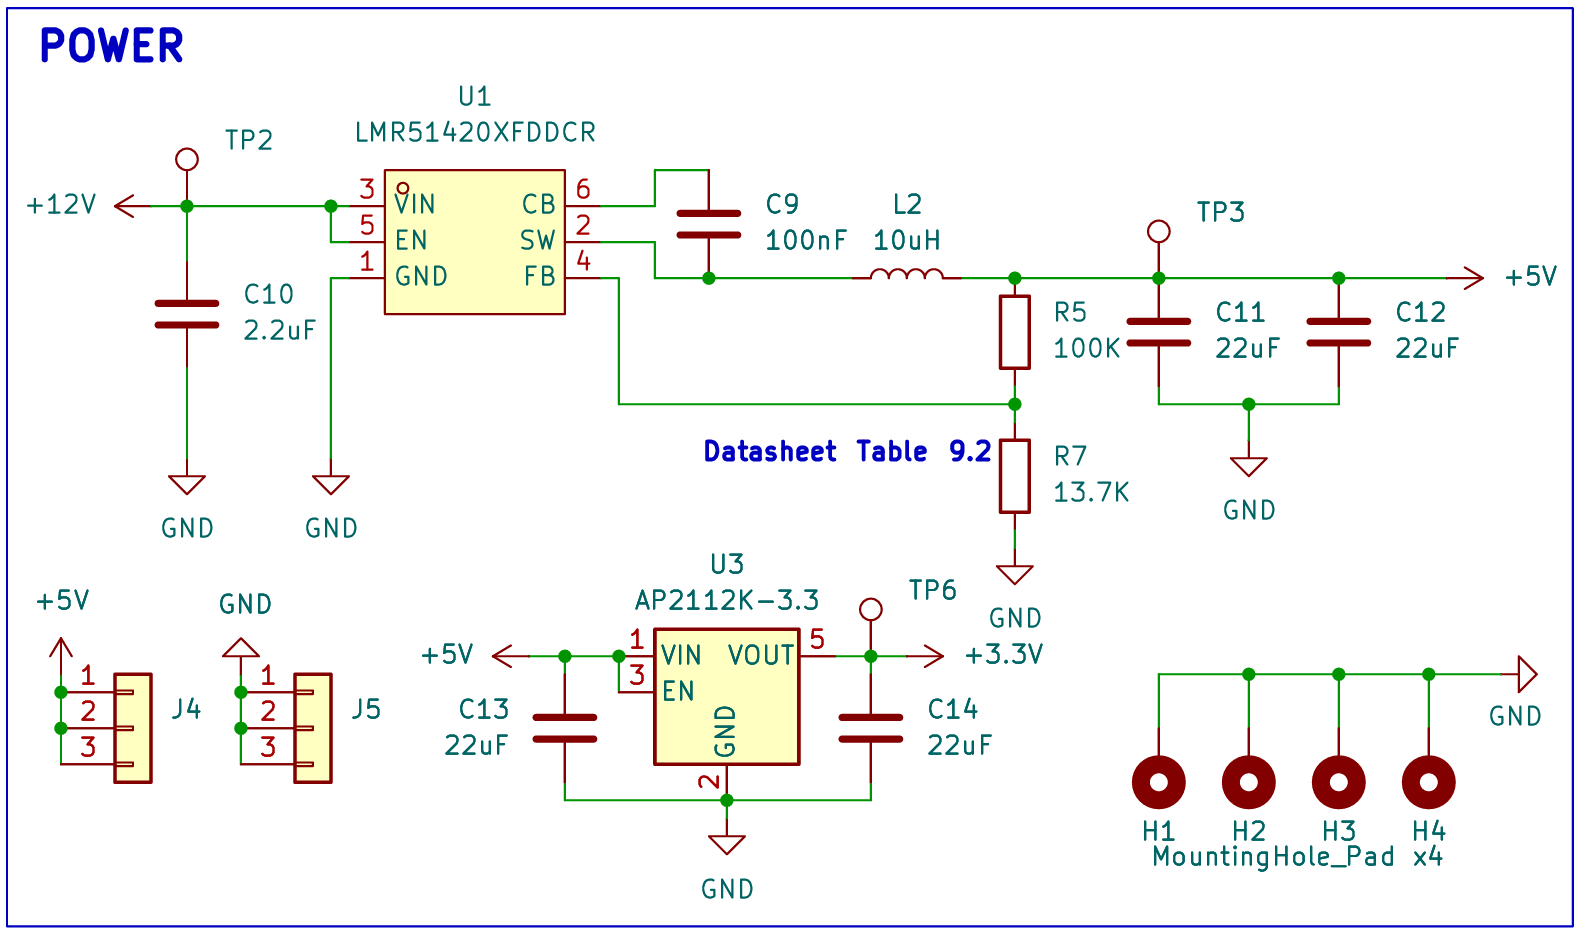
\includegraphics[width=0.9\linewidth]{figures/Power.png}
\caption{Khối nguồn: buck LMR51420 (\SI{12}{\volt}$\to$\SI{5}{\volt}) và LDO AP2112K (\SI{5}{\volt}$\to$\SI{3.3}{\volt})}
\label{fig:sch_power}
\end{figure}

\paragraph{Mạch dao động thạch anh.} Tụ tải C7, C8 = \SI{22}{\pico\farad}; với điện dung ký sinh $C_{stray}\approx\SI{5}{\pico\farad}$, điện dung tải tương đương $C_L=\frac{22\times22}{22+22}+5=\SI{16}{\pico\farad}$, phù hợp với thạch anh \SI{16}{\mega\hertz} thông dụng.

\paragraph{Nguồn tương tự AVCC.} Nguồn +5VA cấp cho AVCC được tách khỏi +5V qua cuộn cảm L1 (\SI{10}{\micro\henry}) / điện trở R1 (\SI{22}{\ohm}) và tụ C3, tạo bộ lọc thông thấp giảm nhiễu chuyển mạch từ buck và cầu H vào ADC. Chân AREF được thoát xuống đất qua C6 (\SI{10}{\nano\farad}).


\begin{figure}[H]
\centering
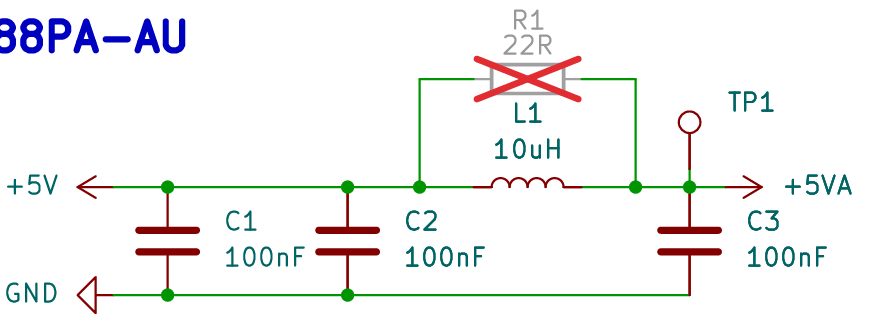
\includegraphics[width=0.6\linewidth]{figures/AVCC.png}
\caption{Bộ lọc nguồn tương tự +5VA cho AVCC}
\label{fig:sch_avcc}
\end{figure}

\paragraph{Nút nhấn.} Nút RUN (SW1) và STOP (SW2) nối lên +5V (tích cực mức cao), có điện trở kéo xuống \SI{10}{\kilo\ohm} và tụ \SI{100}{\nano\farad} tạo bộ lọc RC phần cứng với hằng số thời gian
\begin{equation}
  \tau=RC=10\cdot10^{3}\times100\cdot10^{-9}=\SI{1}{\milli\second},
\end{equation}
kết hợp với bộ chống dội phần mềm \SI{20}{\milli\second} trong firmware.


\begin{figure}[H]
\centering
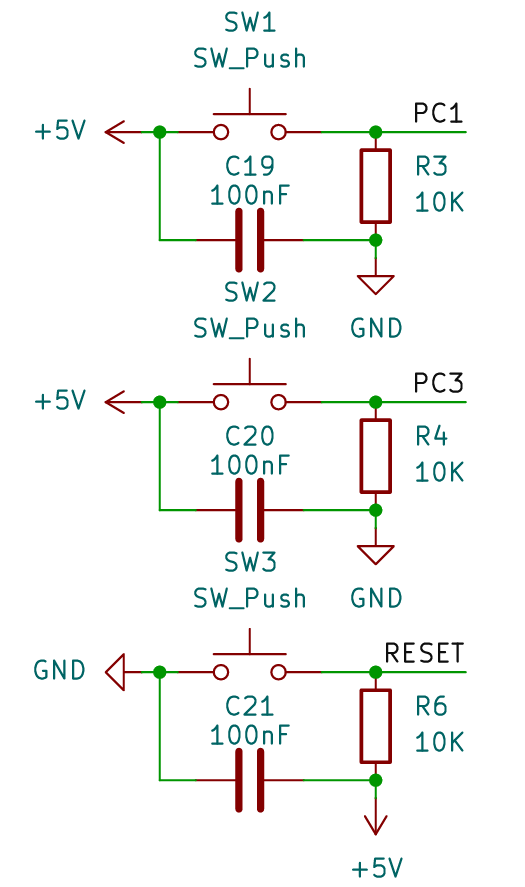
\includegraphics[width=0.35\linewidth]{figures/Button.png}
\caption{Mạch nút nhấn RUN (SW1), STOP (SW2) và RESET (SW3) với bộ lọc RC}
\label{fig:sch_button}
\end{figure}

\paragraph{LED trạng thái.} Mỗi LED được khóa bởi một MOSFET kênh N 2N7002 (Q2, Q3) ở phía thấp; cực cổng nối với chân GPIO qua \SI{22}{\ohm} và kéo xuống \SI{10}{\kilo\ohm} để LED tắt khi MCU đang reset. Dòng qua LED với trở hạn dòng \SI{10}{\kilo\ohm}:
\begin{equation}
  I_{LED}=\frac{V_{CC}-V_F}{R}\approx\frac{5-2}{10\cdot10^{3}}=\SI{0.3}{\milli\ampere},
\end{equation}
đủ sáng để báo hiệu với LED hiệu suất cao và giảm tải cho phần nguồn.

\begin{ghichu}[Vì sao R13 và R16 được đánh dấu DNP?]
Q2, Q3 dùng chung một footprint SOT-23 cho \textbf{hai phương án linh kiện}: MOSFET kênh N (2N7002) hoặc transistor BJT NPN (ví dụ MMBT3904). Hai loại này có sơ đồ chân tương thích trên vỏ SOT-23 (chân 1: G/B, chân 2: S/E, chân 3: D/C), nên có thể thay thế cho nhau mà không phải sửa PCB, tùy linh kiện sẵn có khi lắp ráp. R13 và R16 (\SI{10}{\kilo\ohm}, nối cực điều khiển xuống GND) chỉ cần thiết với một trong hai phương án, nên mặc định được đánh dấu \textbf{DNP} (\emph{Do Not Populate} -- không hàn) và chỉ hàn khi cần, đúng như ghi chú trên sơ đồ nguyên lý: \emph{``Solder R13 and R16 when Q2 and Q3 are MOSFETs''}.
\end{ghichu}


\begin{figure}[H]
\centering
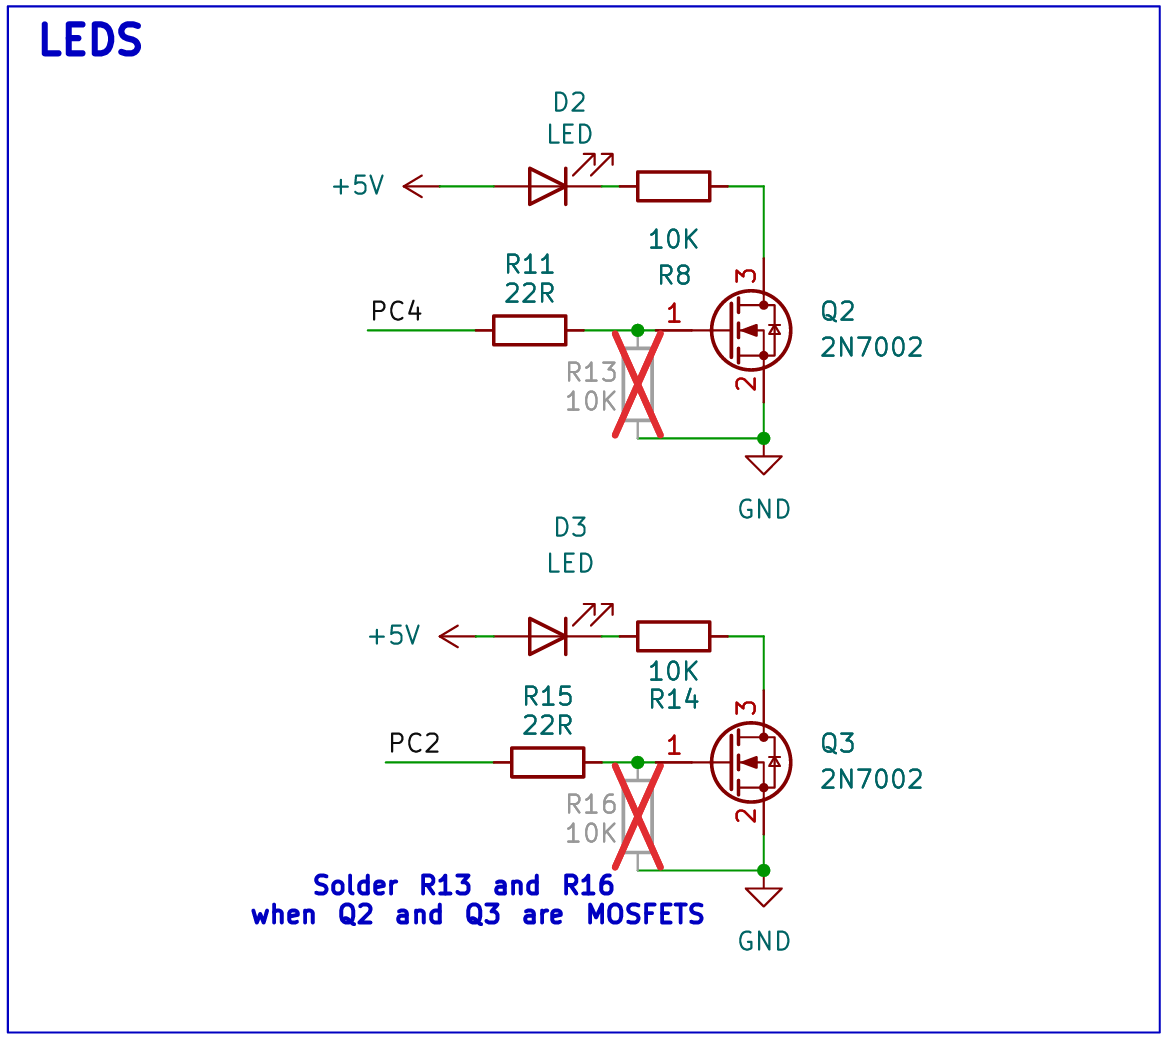
\includegraphics[width=0.7\linewidth]{figures/LEDs.png}
\caption{Mạch LED trạng thái khóa bằng MOSFET 2N7002}
\label{fig:sch_leds}
\end{figure}

\paragraph{Cổng nạp và Test point.} Đầu nối J6 (RESET, MOSI, MISO, SCK, GND) cho phép nạp ISP. Bảy Test point TP1--TP7 được đặt tại các nút quan trọng: +5VA, +12V, +5V, ENC\_A, ENC\_B, +3.3V và OE -- phục vụ trực tiếp việc đo kiểm ở Chương~\ref{ch:lapdat}.

\section{Thiết kế mạch in (PCB)}

\subsection{Thông số bo mạch}
\begin{table}[H]
\centering\small
\caption{Thông số chế tạo PCB}
\label{tab:pcbspec}
\begin{tabular}{@{}ll@{}}
\toprule
\textbf{Thông số} & \textbf{Giá trị}\\
\midrule
Kích thước & 80\,$\times$\,60\,mm\\
Số lớp đồng & 2 (F.Cu, B.Cu)\\
Độ dày bo & \SI{1.6}{\milli\metre} FR-4\\
Độ rộng đường tín hiệu & \SIrange{0.2}{0.3}{\milli\metre}\\
Độ rộng đường nguồn & \SI{0.5}{\milli\metre} và đổ đồng (copper pour)\\
Số via & 280 (bao gồm via khâu mặt đất và via tản nhiệt)\\
Lỗ bắt vít & 4 $\times$ M3, có pad nối GND\\
Gia công & Đặt sản xuất tại JLCPCB từ tệp Gerber xuất từ KiCad\\
\bottomrule
\end{tabular}
\end{table}

\subsection{Bố trí linh kiện (placement)}
Bo mạch được chia thành các vùng chức năng rõ ràng nhằm tách biệt dòng công suất khỏi tín hiệu nhạy cảm:
\begin{itemize}
  \item \textbf{Vùng nguồn} (cạnh trái): đầu vào J1, MOSFET chống ngược cực Q1, buck U1, LDO U3 và các tụ bulk. Đầu nối nguồn đặt ở mép bo để dễ đấu dây (Hình~\ref{fig:place_power}).
  \item \textbf{Vùng công suất} (góc trên bên phải): DRV8220 (U5), jumper chọn chế độ JP1 và domino động cơ M1 ở mép phải -- đường dòng động cơ ngắn và nằm xa vùng tương tự (Hình~\ref{fig:place_motor}).
  \item \textbf{Vùng vi điều khiển} (trung tâm): ATmega88PA (U2) với thạch anh Y1 đặt sát chân XTAL1/\allowbreak XTAL2, các tụ thoát \SI{100}{\nano\farad} đặt sát từng chân cấp nguồn; cổng nạp J6 ngay phía trên MCU (Hình~\ref{fig:place_mcu}).
  \item \textbf{Vùng giao diện}: header màn hình J2 và IC chuyển mức U4 ở bên trái -- màn hình cắm chồng lên bo; chiết áp RV1, nút RUN/STOP/RESET và LED xếp dọc cạnh dưới để người dùng thao tác; đầu JST encoder J7 và UART J3 gom về cạnh phải (Hình~\ref{fig:place_ui}).
\end{itemize}

\begin{figure}[H]
\centering
\begin{subfigure}{0.65\linewidth}\centering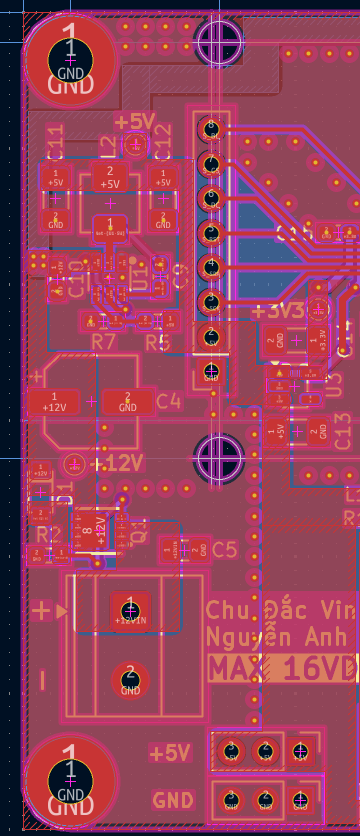
\includegraphics[angle=90,width=\linewidth]{figures/Power_Layout.png}\caption{Layout}\end{subfigure}

\vspace{0.5em}
\begin{subfigure}{0.65\linewidth}\centering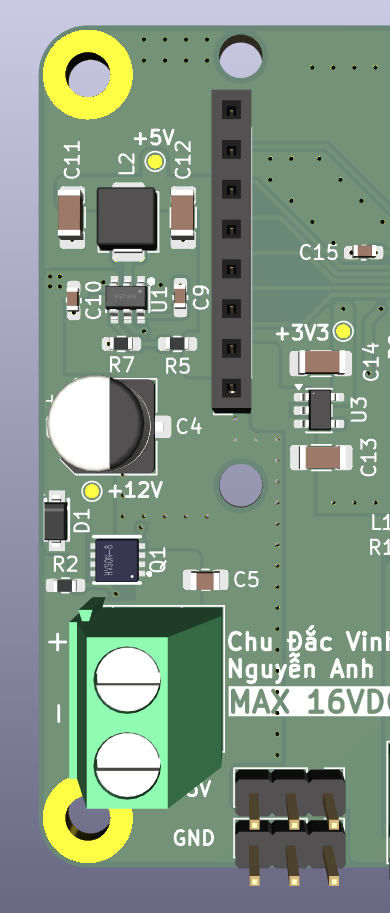
\includegraphics[angle=90,width=\linewidth]{figures/Power_3D.png}\caption{Ảnh 3D}\end{subfigure}
\caption{Bố trí linh kiện vùng nguồn}
\label{fig:place_power}
\end{figure}

\begin{figure}[H]
\centering
\begin{subfigure}{0.65\linewidth}\centering\hinh[\linewidth]{figures/Motor_Driver_Layout.png}{Layout vùng công suất (cầu H DRV8220)}\caption{Layout}\end{subfigure}

\vspace{0.5em}
\begin{subfigure}{0.65\linewidth}\centering\hinh[\linewidth]{figures/Motor_Driver_3D.png}{Ảnh 3D vùng công suất (cầu H DRV8220)}\caption{Ảnh 3D}\end{subfigure}
\caption{Bố trí linh kiện vùng công suất (cầu H DRV8220)}
\label{fig:place_motor}
\end{figure}

\begin{figure}[H]
\centering
\begin{subfigure}{0.49\linewidth}\centering\hinh[\linewidth]{figures/MCU_Layout.png}{Layout vùng vi điều khiển}\caption{Layout}\end{subfigure}
\hfill
\begin{subfigure}{0.49\linewidth}\centering\hinh[\linewidth]{figures/MCU_3D.png}{Ảnh 3D vùng vi điều khiển}\caption{Ảnh 3D}\end{subfigure}
\caption{Bố trí linh kiện vùng vi điều khiển}
\label{fig:place_mcu}
\end{figure}

\begin{figure}[H]
\centering
\begin{subfigure}{0.65\linewidth}\centering\hinh[\linewidth]{figures/UI_Layout.png}{Layout vùng giao diện người dùng}\caption{Layout}\end{subfigure}

\vspace{0.5em}
\begin{subfigure}{0.65\linewidth}\centering\hinh[\linewidth]{figures/UI_3D.png}{Ảnh 3D vùng giao diện người dùng}\caption{Ảnh 3D}\end{subfigure}
\caption{Bố trí linh kiện vùng giao diện người dùng}
\label{fig:place_ui}
\end{figure}

\subsection{Đi dây (routing)}
\begin{itemize}
  \item \textbf{Vòng chuyển mạch buck} (VIN -- tụ vào -- chân SW -- cuộn cảm -- tụ ra -- GND) được giữ ngắn và nhỏ nhất có thể để giảm bức xạ nhiễu điện từ, tụ vào C10 đặt sát chân VIN/GND của U1.
  \item \textbf{Đường dòng động cơ} (VM, OUT1, OUT2) dùng đường rộng \SI{0.5}{\milli\metre} và vùng đổ đồng; pad tản nhiệt (exposed pad) của DRV8220 được khâu xuống mặt dưới bằng nhiều via.
  \item \textbf{Mặt đất và vùng đồng nguồn}: GND được đổ đồng trên cả hai lớp; các vùng đồng riêng cho +12V, +5V, +5VA, +3.3V và OUT1/OUT2 nằm ở lớp trên. Phần lớn đường tín hiệu đi ở lớp trên (210/250 đoạn dây) để mặt đất lớp dưới ít bị cắt; các via khâu (stitching via) nối đồng GND hai lớp.
  \item \textbf{Đường tín hiệu nhạy}: đường encoder và ADC chiết áp đi xa vùng chuyển mạch; đường SPI tới TFT đi ngắn qua TXB0106.
\end{itemize}

\begin{figure}[H]
\centering
\begin{subfigure}{0.49\linewidth}\centering\hinh[\linewidth]{figures/Layout_Front.png}{Layout lớp trên}\caption{Lớp trên (F.Cu)}\end{subfigure}
\hfill
\begin{subfigure}{0.49\linewidth}\centering\hinh[\linewidth]{figures/Layout_Back.png}{Layout lớp dưới}\caption{Lớp dưới (B.Cu)}\end{subfigure}
\caption{Layout mạch in \proj}
\label{fig:layout}
\end{figure}

\subsection{Kiểm tra và xuất tệp sản xuất}
Trước khi đặt gia công, thiết kế được kiểm tra bằng ERC (Electrical Rules Check) cho sơ đồ nguyên lý và DRC (Design Rules Check) cho PCB theo năng lực công nghệ của nhà sản xuất (đường/khoảng cách tối thiểu \SI{0.15}{\milli\metre}, lỗ khoan tối thiểu \SI{0.3}{\milli\metre}). Bộ tệp sản xuất gồm Gerber các lớp đồng, mặt nạ hàn, lụa, kem hàn, đường viền bo (Edge.Cuts) và tệp khoan Excellon (\texttt{.drl}).

Trước khi gửi đi gia công, bộ tệp Gerber được mở lại bằng trình xem Gerber (Gerber Viewer) để kiểm tra lần cuối: các lớp đồng, mặt nạ hàn, lụa và lỗ khoan phải chồng khớp nhau, đường viền bo khép kín và không có lớp nào bị thiếu hoặc lệch so với thiết kế (Hình~\ref{fig:gerber}).

\begin{figure}[H]
\centering
\hinh[0.85\linewidth]{figures/Gerber_Viewer.png}{Kiểm tra bộ tệp Gerber trên trình xem Gerber}
\caption{Kiểm tra bộ tệp sản xuất trên Gerber Viewer}
\label{fig:gerber}
\end{figure}

\subsubsection{Dụng cụ hàn linh kiện}
Sau khi nhận bo mạch trần, linh kiện được hàn thủ công tại chỗ. Do phần lớn linh kiện là loại dán bề mặt (SMD) với bước chân nhỏ, phương pháp chính là quét kem hàn lên pad rồi dùng khí nóng để nung chảy (hot-air reflow); mỏ hàn chỉ dùng cho linh kiện xuyên lỗ và sửa mối hàn. Các dụng cụ được sử dụng được liệt kê ở Bảng~\ref{tab:solder_equipment} và Hình~\ref{fig:solder_equipment}.

\begin{table}[H]
\centering
\caption{Dụng cụ hàn và lắp ráp linh kiện}
\label{tab:solder_equipment}
\begin{tabularx}{\linewidth}{|l|X|}
\hline
\textbf{Dụng cụ} & \textbf{Công dụng} \\
\hline
Kem hàn Relife RL-403S & Kem hàn dạng ống tiêm \SI{10}{cc}, nhiệt độ nóng chảy \SI{183}{\celsius}; được bơm trực tiếp lên từng pad SMD trước khi đặt linh kiện. \\
\hline
Súng bơm kem hàn Relife RL-062A & Gắn với ống kem hàn RL-403S, giúp định lượng và đưa kem hàn lên pad chính xác, đều tay. \\
\hline
Trạm khò hàn AIFEN 868D & Thổi khí nóng để nung chảy kem hàn (reflow) cho các linh kiện SMD như IC, điện trở, tụ điện; đồng thời dùng để tháo linh kiện khi cần sửa. \\
\hline
Trạm hàn SUNSHINE S3 & Mỏ hàn dùng để hàn linh kiện xuyên lỗ (header, domino, đầu nối), sửa mối hàn thiếu thiếc hoặc bị dính chân (bridge). \\
\hline
Nhíp Relife SA-11 & Gắp, đặt và căn chỉnh linh kiện SMD lên vị trí trước và trong khi khò. \\
\hline
\end{tabularx}
\end{table}

Quy trình hàn được thực hiện theo thứ tự: (1) bơm kem hàn lên các pad bằng súng RL-062A; (2) dùng nhíp SA-11 đặt linh kiện SMD vào đúng vị trí và chiều; (3) khò bằng trạm AIFEN 868D tới khi kem hàn chảy và linh kiện tự căn chỉnh vào pad nhờ sức căng bề mặt; (4) hàn các linh kiện xuyên lỗ và kiểm tra, sửa mối hàn bằng trạm hàn SUNSHINE S3.

\begin{figure}[H]
\centering
\hinh[0.8\linewidth]{figures/solder_equipment.png}{Ảnh các dụng cụ hàn linh kiện}
\caption{Các dụng cụ dùng để hàn linh kiện}
\label{fig:solder_equipment}
\end{figure}

\begin{figure}[H]
\centering
\hinh[0.7\linewidth]{figures/pcb_thucte.jpg}{Ảnh chụp bo mạch thực tế sau khi hàn linh kiện}
\caption{Bo mạch \proj{} sau khi lắp ráp}
\label{fig:pcbthucte}
\end{figure}
